\documentclass[11pt,a4paper]{article}

\usepackage[margin=1in]{geometry}
\usepackage{lmodern}
\usepackage[T1]{fontenc}
\usepackage[utf8]{inputenc}
\usepackage{microtype}
\usepackage{setspace}
\usepackage{booktabs}
\usepackage{tabularx}
\usepackage{graphicx}
\usepackage{caption}
\usepackage{amsmath}
\usepackage{amssymb}
\usepackage{enumitem}
\usepackage[hyphens]{url}
\usepackage[hidelinks]{hyperref}
\usepackage{xcolor}
\usepackage{titlesec}

\onehalfspacing
\setlength{\parskip}{0.35em}
\setlength{\parindent}{0pt}
\setlist[itemize]{leftmargin=1.4em,itemsep=0.15em,topsep=0.25em}
\setlist[enumerate]{leftmargin=1.4em,itemsep=0.15em,topsep=0.25em}
\captionsetup{font=small,labelfont=bf,skip=6pt}
\titleformat{\section}{\large\bfseries}{\thesection.}{0.6em}{}
\titleformat{\subsection}{\normalsize\bfseries}{\thesubsection}{0.5em}{}

\newcommand{\lab}{Monterey Finance Halal Quant Research Lab}
\newcommand{\strat}{Halal FCF quality}

\title{%
  Cash Generation under AAOIFI Debt Limits:\\
  An Exploratory Backtest of Halal FCF Quality, 2023--2024}
\author{\lab\\Paper 01 \textperiodcentered{} Exploratory note}
\date{August 2026}

\begin{document}
\maketitle

\begin{abstract}
\noindent
This is an internal exploratory note, not a finished proof and not a live-return target.
In the two calendar years 2023--2024, a cap-weighted basket of AAOIFI-screened S\&P~500 names with free-cash-flow (FCF) margins in the top half of that month returned \textbf{42.4\%} compound annual growth, versus \textbf{25.9\%} for the S\&P~500 (SPY) and \textbf{31.1\%} for a Halal large-cap ETF (SPUS).
The live rule is cash generation, not cheapness: after banned businesses and the AAOIFI debt cap, we keep names that convert a large share of sales into free cash flow and own them in proportion to company size.
The book is a Halal mega-cap quality/tech portfolio. Technology plus communication services averaged about 74\% of weight. Much of the win is that tilt in a mega-cap boom, not a cycle-proof quality premium.
A prior cheapness rule (FCF/enterprise value) was dropped after it missed Apple and Nvidia and lost to SPUS. That change used the same 2023--2024 window, so these results are partly in-sample.
\end{abstract}

\tableofcontents
\vspace{1em}
\noindent\textit{Status.} Exploratory. Reproduce from \texttt{code.ipynb}. Figures in \texttt{figures/}. Sharia screens are a hard point-in-time constraint, not an overlay.

%----------------------------------------------------------------------
\section{Hypothesis \& Theory}

\subsection{What we are testing}

The lab backlog item for this paper was enterprise-value cash-flow yield (FCF/EV) paired with AAOIFI leverage limits, to see whether a 30\% debt cap leaves a cleaner ``quality'' book than the broad market~\cite{aaoifi21}.
The first implementation ranked by cheapness (high FCF/EV) and equal-weighted the top fifth.
That book lost to SPUS in 2023--2024 because Apple and Nvidia passed the Halal screens but looked \emph{expensive} on FCF/EV, so they were not bought, while SPUS is a broad, cap-weighted Halal basket that owned the mega-cap winners.

The live rule in this note is therefore different. The economic claim is simpler:

\begin{quote}
After dropping banned businesses and names above the AAOIFI debt cap, do companies that \textbf{actually generate cash} (high free cash flow versus sales) hold up as a Halal equity book, when owned in proportion to size?
\end{quote}

Cheapness is not used to pick or weight names. FCF/EV is stored only as a diagnostic.

\subsection{Why cash generation and debt caps might interact}

Free cash flow is cash from operations minus capital spending. FCF margin is that cash divided by sales. A high margin means the business turns a large share of revenue into cash after reinvestment. That is a quality signal, not a value signal.

AAOIFI financial screens cap interest-bearing debt, cash, and receivables relative to market value. In this test the debt rule is total debt below 30\% of trailing 24-month market cap, plus the library's cash and receivables screens. The hypothesis is that those caps remove highly leveraged firms and leave a pool where cash generation is more informative---or at least not cancelled out by balance-sheet distress.

We do \emph{not} claim that the debt cap ``creates'' a quality premium by itself. The 2023--2024 sample is too short and too tech-heavy to separate the screen from the sector mix.

\subsection{Universe and screening standard}

\begin{center}
\begin{tabular}{ll}
\toprule
Item & Choice \\
\midrule
Target factor & FCF margin $=$ free cash flow / sales \\
Starting universe & Current S\&P~500 list (503 tickers) \\
After banned-business screen & 439 tickers (64 removed) \\
Screening standard & AAOIFI financial ratios, not DJIM \\
Halal benchmark & SPUS (SP Funds S\&P~500 Sharia Industry Exclusions) \\
All-stock benchmark & SPY (S\&P~500) \\
Sample requested & 1~Jan~2019 -- 31~Dec~2024 \\
Live window used for stats & 3~Jan~2023 -- 30~Dec~2024 (501 trading days) \\
\bottomrule
\end{tabular}
\end{center}

Sector exclusions (banks, conventional insurance, alcohol, tobacco, gambling, weapons, and similar) run once on the current constituent list. Debt, cash, and receivables screens re-run at every month-end on point-in-time filings.

SPUS is the Halal \emph{index} comparison required by the lab template. It is not identical to AAOIFI: it is an industry-exclusion ETF, cap-weighted, with its own reconstitution calendar. Beating SPUS is not the same as beating a pure AAOIFI financial-ratio index, and we do not have a DJIM-tracking book in this run.

Yahoo had no price history in-sample for Q, SNDK, and FDXF (names listed after 2024). They are skipped.

\subsection{What would count as a finished proof}

This note would move from ``exploratory'' to ``ready for a live mandate'' only after: a frozen rule, ten to fifteen years of SEC cash-flow tags, point-in-time S\&P membership, at least one down year like 2022, a sector-capped twin, and a hold-out window that was not used to rewrite the rule. None of that is in this file.

%----------------------------------------------------------------------
\section{Strategy Rules}

Rules are unambiguous and applied with no look-ahead. Compliance is a hard constraint: a name that fails on a rebalance date is not held.

\subsection{Pipeline at each month-end}

\begin{enumerate}
  \item \textbf{Start} from the sector-eligible S\&P~500 list (439 names).
  \item \textbf{Filter (AAOIFI).} Drop names that fail debt / 24-month market cap $< 30\%$, or the cash and receivables screens, using filings known as of that date (\texttt{filed\_date}, or report date plus 90 days).
  \item \textbf{Score.} Compute FCF margin $=$ FCF / sales. Require FCF $> 0$. FCF comes from yfinance annual cash-flow statements with a 90-day publication lag.
  \item \textbf{Select.} Keep the top half of that Halal list by FCF margin (\texttt{KEEP\_QUANTILE} $= 0.50$).
  \item \textbf{Weight.} Cap-weight by market cap. No equal-weight, no inverse-vol, no optimizer.
  \item \textbf{Rebalance.} Repeat at month-end (\texttt{REBALANCE\_FREQ} $=$ \texttt{ME}).
\end{enumerate}

If fewer than 20 names survive (\texttt{MIN\_HOLDINGS}), that month is skipped and the book stays in cash (treated as missing, not as a 0\% return). Performance statistics start on the first day the strategy actually holds stocks, not on the 2019 start date.

\subsection{Entry, exit, and risk limits}

\begin{center}
\begin{tabular}{ll}
\toprule
Rule & Specification \\
\midrule
Entry & Halal + FCF $> 0$ + FCF margin in the top half that month \\
Exit & Sold at the next month-end if the name fails AAOIFI, \\
     & loses positive FCF, or drops out of the top half \\
Intra-month stop-loss & None \\
Position cap & None beyond cap-weight \\
Cash when thin & Skip the month if holdings $< 20$ \\
Robustness twin & Same screen, then drop the jumpiest fifth \\
     & of those picks (252-day volatility) \\
\bottomrule
\end{tabular}
\end{center}

There is no stop-loss and no single-name cap. At the last rebalance (31~Dec~2024) Apple was 13.4\%, Nvidia 11.9\%, Microsoft 11.1\%, and the two Alphabet share classes together were about 16.8\%. That is a concentrated mega-cap book by design.

\subsection{Holdings through time}

Median live book size is 124 names (min~20, max~130). Early months sit on the 20-name floor; coverage then jumps and stays in the 120--130 range through 2024. The funnel at a typical month is: about 419 names with fundamentals, 233 Halal with positive FCF, 116 actually bought.

\begin{figure}[htbp]
\centering
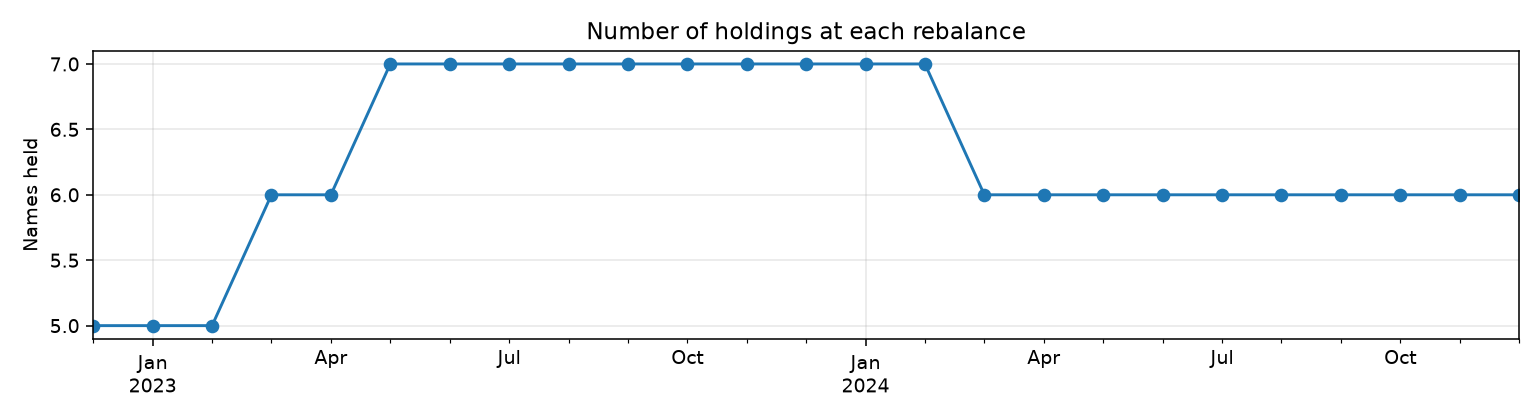
\includegraphics[width=0.92\textwidth]{figures/holdings-count.png}
\caption{Number of names held at each month-end. The 20-name floor binds in late 2022 / early 2023; the book then becomes a broad, cap-weighted quality slice of the Halal S\&P list.}
\label{fig:holdings}
\end{figure}

\subsection{Names that enter, stay, or leave}

Sharia status and the FCF-margin rank are re-checked every month. A held name that fails is exited at that rebalance---not left in the book until a human review.

On 31~Dec~2024 the watchlist split as follows:

\begin{itemize}
  \item \textbf{Held:} AAPL, NVDA, MSFT, GOOGL, META, AVGO. All Halal-ok, all in the top half by FCF margin. Apple's FCF yield was only 2.8\% (expensive on the old cheapness rule) with a 27.8\% FCF margin (kept under the live rule).
  \item \textbf{Halal-ok but not bought:} AMZN (FCF-margin rank 224 of 255) and TSLA (rank 234 of 255). The screen keeps about 128 names; both sat in the bottom half.
  \item \textbf{Not bought --- no positive FCF:} LLY that month (FCF margin $-9.2\%$). Lilly was held in 12 of 38 metric months when FCF was positive and high enough.
\end{itemize}

Amazon and Tesla were never in the live book (0 of 38 months). That is the cash-generation screen working as written, not a data accident at the last date. Microsoft and Nvidia show ``data gap'' months in the autopsy: Yahoo/SEC snapshots were missing for some month-ends, so the name was skipped that month even if it would have passed.

GOOG and GOOGL were both held as separate lines. Cap-weighting two share classes of the same company inflates Alphabet relative to a single-listing index. That is a construction bug to fix in a follow-up, not a feature.

%----------------------------------------------------------------------
\section{Empirical Performance}

All headline numbers use the \textbf{live window} only: 3~January~2023 through 30~December~2024 (501 trading days). Days before the first invested date are omitted, not filled with zeros. Yahoo's short FCF history is why the book does not go live in 2019.

\subsection{Headline results}

\begin{table}[htbp]
\centering
\caption{Live-window performance, 3~Jan~2023 -- 30~Dec~2024. Sharpe and Sortino use a 2\% risk-free rate. Max drawdown is peak-to-trough on the growth curve.}
\label{tab:perf}
\small
\begin{tabular}{lrrrrrr}
\toprule
Book & CAGR & Vol. & Sharpe & Sortino & Max DD & Calmar \\
\midrule
Halal FCF quality           & 42.43\% & 16.13\% & 2.15 & 3.10 & $-11.92\%$ & 3.56 \\
Quality (drop high vol)     & 34.26\% & 14.45\% & 1.97 & 2.85 & $-9.39\%$  & 3.65 \\
S\&P~500 (SPY)              & 25.93\% & 12.82\% & 1.71 & 2.50 & $-9.97\%$  & 2.60 \\
Halal (SPUS)                & 31.11\% & 15.07\% & 1.74 & 2.58 & $-11.46\%$ & 2.71 \\
\bottomrule
\end{tabular}
\end{table}

The quality book beat both required benchmarks on CAGR, Sharpe, Sortino, and Calmar. It took a slightly deeper drawdown than SPY ($-11.9\%$ vs $-10.0\%$) and a similar one to SPUS. Dropping the jumpiest fifth of the quality names cut CAGR to 34.3\% but also cut volatility and drawdown; Calmar stayed similar (3.65 vs 3.56). That overlay still beat SPY and SPUS. It is a robustness check, not a second live product.

These CAGRs are two-year annualized figures from a mega-cap bull market. They are not a forecast of 42\% a year.

\begin{figure}[htbp]
\centering
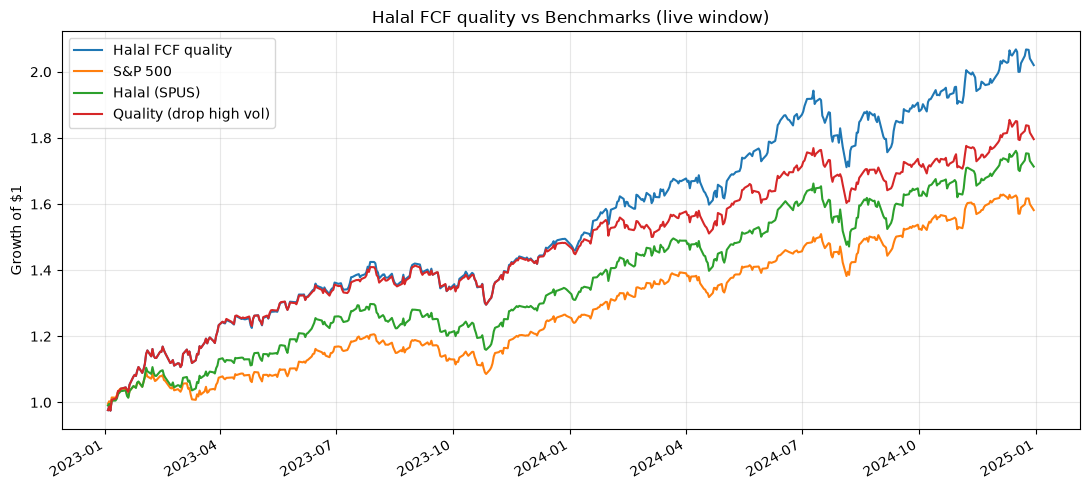
\includegraphics[width=0.92\textwidth]{figures/equity-curves.png}
\caption{Growth of \$1 in the live window. The quality book finishes near \$2.00, the low-vol overlay near \$1.80, SPUS near \$1.70, and SPY near \$1.60.}
\label{fig:equity}
\end{figure}

\subsection{Calendar years}

\begin{table}[htbp]
\centering
\caption{Calendar-year total returns inside the live window.}
\label{tab:calendar}
\begin{tabular}{lrrr}
\toprule
Year & Halal FCF quality & S\&P~500 & Halal (SPUS) \\
\midrule
2023 & 49.12\% & 26.18\% & 34.20\% \\
2024 & 35.47\% & 25.34\% & 27.67\% \\
\bottomrule
\end{tabular}
\end{table}

The quality book led in both years: by about 23 points vs SPY and 15 vs SPUS in 2023, and by about 10 and 8 points in 2024. There is no down year in this sample.

\begin{figure}[htbp]
\centering
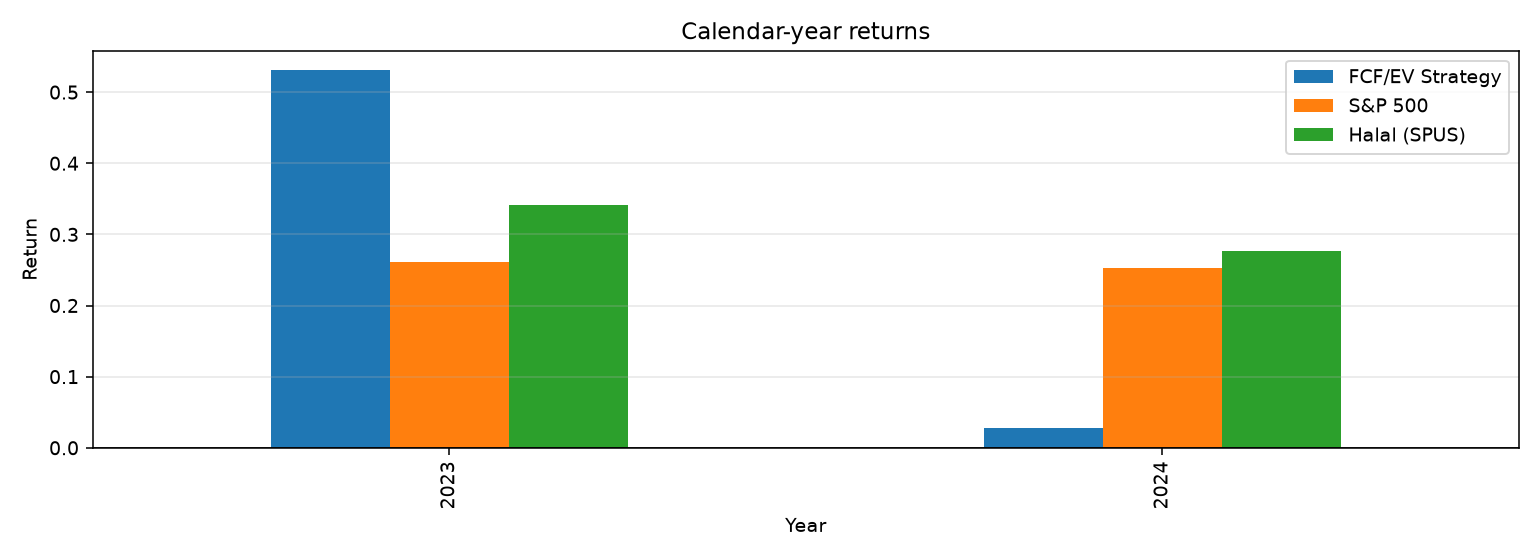
\includegraphics[width=0.92\textwidth]{figures/calendar-year-returns.png}
\caption{Calendar-year returns. The quality book is the tallest bar in both 2023 and 2024.}
\label{fig:calendar}
\end{figure}

\begin{figure}[htbp]
\centering
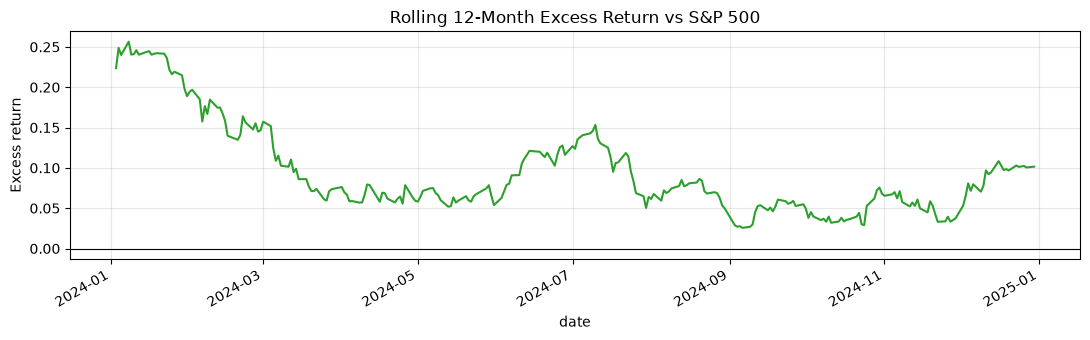
\includegraphics[width=0.92\textwidth]{figures/rolling-excess.png}
\caption{Rolling 12-month excess return versus SPY. Excess stayed positive through the live window, starting near $+25\%$ in early 2024 and ending near $+10\%$.}
\label{fig:excess}
\end{figure}

\subsection{Drawdowns}

\begin{figure}[htbp]
\centering
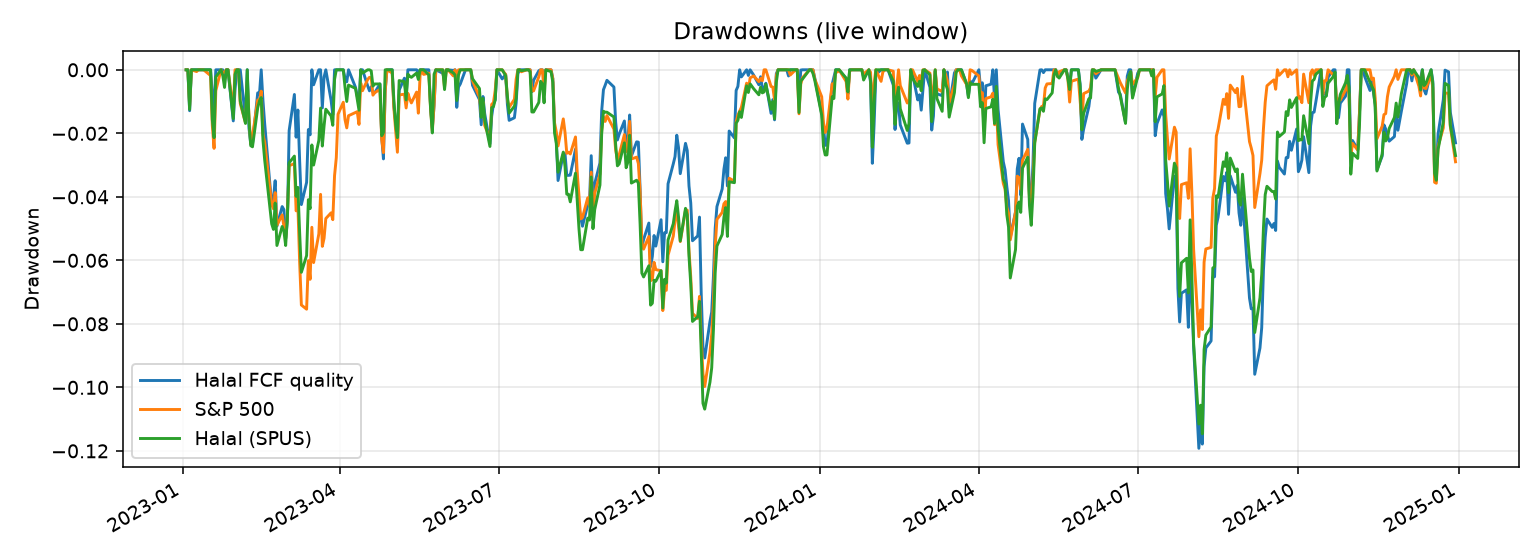
\includegraphics[width=0.92\textwidth]{figures/drawdowns.png}
\caption{Drawdowns in the live window. Paths track SPUS more closely than SPY. The quality book's worst mark (about $-11.9\%$) is in mid-2024, when Halal/tech names sold off harder than the full S\&P~500.}
\label{fig:dd}
\end{figure}

The quality book and SPUS dip together in late 2023, mid-2024, and late 2024. SPY's mid-2024 drawdown is shallower. That is consistent with a Halal mega-cap tech book, not with a defensive quality book.

\subsection{Does higher FCF margin actually pay?}

Inside the same Halal universe we cap-weight five FCF-margin buckets. Q1 is the highest cash generation; Q5 is the lowest. The live strategy is roughly the top half (near Q1--Q2), not a single quintile.

\begin{table}[htbp]
\centering
\caption{Cap-weighted FCF-margin quintiles inside the Halal universe, live window. Q1 $=$ highest FCF/sales.}
\label{tab:quintiles}
\small
\begin{tabular}{lrrrrrr}
\toprule
Bucket & CAGR & Vol. & Sharpe & Sortino & Max DD & Calmar \\
\midrule
Q1 & 37.44\% & 19.34\% & 1.64 & 2.35 & $-15.14\%$ & 2.47 \\
Q2 & 35.76\% & 16.34\% & 1.83 & 2.48 & $-10.03\%$ & 3.57 \\
Q3 & 27.39\% & 16.86\% & 1.40 & 2.26 & $-13.08\%$ & 2.09 \\
Q4 & 11.62\% & 14.96\% & 0.68 & 1.14 & $-14.16\%$ & 0.82 \\
Q5 & 31.08\% & 15.07\% & 1.74 & 2.60 & $-11.74\%$ & 2.65 \\
\bottomrule
\end{tabular}
\end{table}

Q1 and Q2 are the two best CAGRs, which supports keeping the top half. The pattern is \textbf{not} perfectly monotonic: Q5 beat Q3 and Q4. Q2 had the best Sharpe and Calmar. Q1$-$Q5 annualized spread was 5.5\%, with Q1 beating Q5 on 51.3\% of days. The cumulative spread ended near $+10\%$ after peaking around 1.28.

Cash generation helped in this window. It did not line up as a clean, stair-step factor.

\begin{figure}[htbp]
\centering
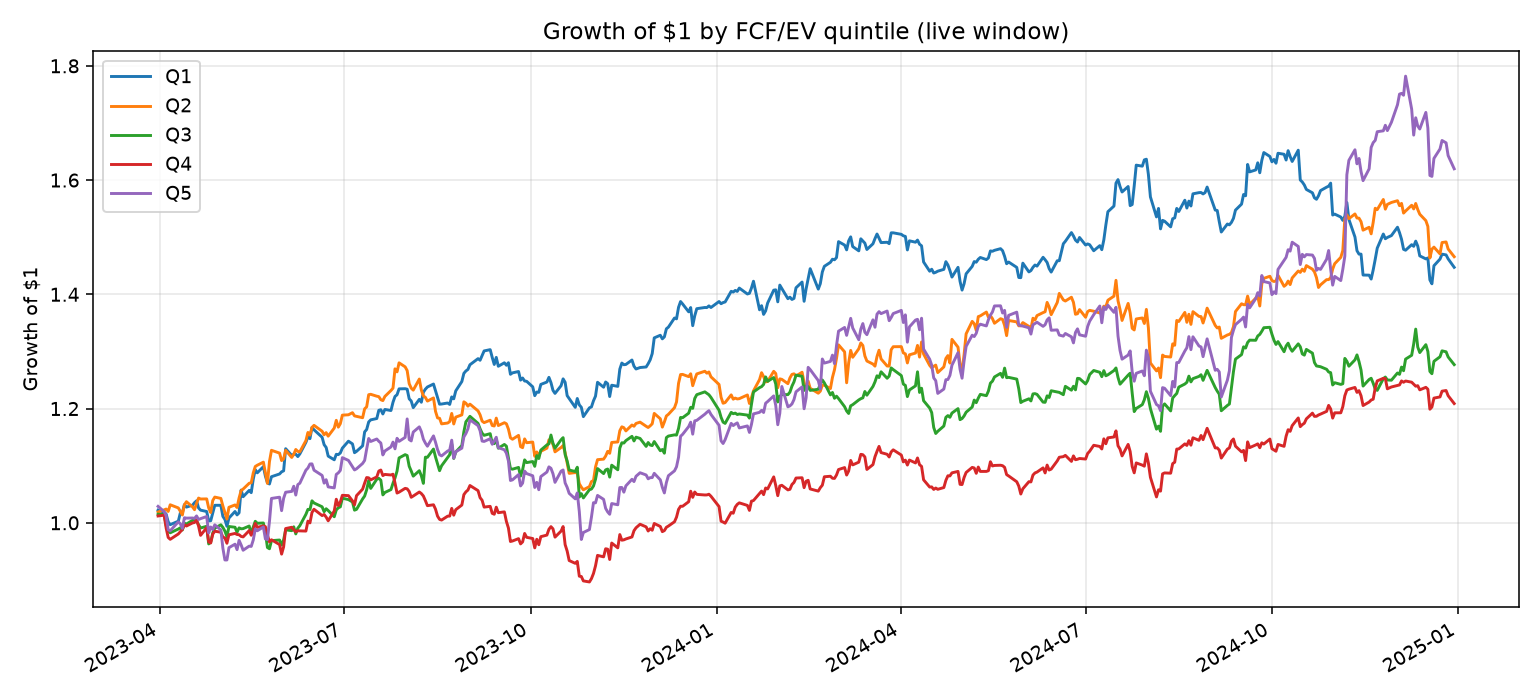
\includegraphics[width=0.92\textwidth]{figures/quintile-growth.png}
\caption{Growth of \$1 by FCF-margin quintile. Q1 and Q2 lead; Q4 lags; Q5 is not last.}
\label{fig:qgrowth}
\end{figure}

\begin{figure}[htbp]
\centering
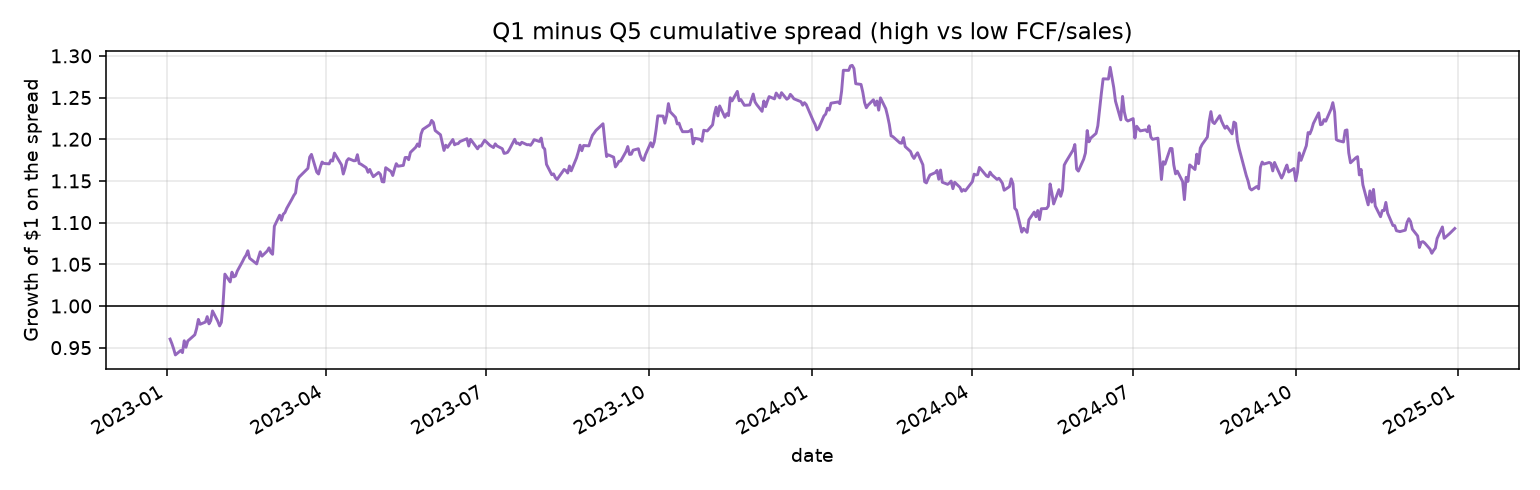
\includegraphics[width=0.92\textwidth]{figures/quintile-spread.png}
\caption{Cumulative Q1 minus Q5 spread. After early 2023 the line stays above 1, but it is noisy and faded from a peak near 1.28 to about 1.10 by the end of 2024.}
\label{fig:qspread}
\end{figure}

%----------------------------------------------------------------------
\section{Factor Attribution}

Section~3 shows the book won. This section asks whether that win is stock picking or a hidden sector bet.

\subsection{Alpha, beta, tracking error}

Daily excess returns of the quality book are regressed on each benchmark (CAPM-style, 2\% risk-free rate). Alpha is annualized.

\begin{table}[htbp]
\centering
\caption{Halal FCF quality versus each benchmark, live window.}
\label{tab:capm}
\begin{tabular}{lrrrrr}
\toprule
Benchmark & Alpha (ann.) & Beta & $R^2$ & Tracking error & Info.\ ratio \\
\midrule
S\&P~500     & 9.56\% & 1.15 & 0.83 & 6.86\% & 1.87 \\
Halal (SPUS) & 7.97\% & 1.02 & 0.91 & 4.95\% & 1.71 \\
\bottomrule
\end{tabular}
\end{table}

Versus SPY the book is a bit more aggressive ($\beta = 1.15$) with 9.6\% leftover annualized alpha and 6.9\% tracking error. Versus SPUS it is almost a parallel book: $\beta = 1.02$, $R^2 = 0.91$, tracking error 5.0\%, still 8.0\% alpha. In plain language: \textbf{this is an SPUS-like Halal large-cap book with extra mega-cap tech}, not an independent style that wiggles on its own.

The information ratios (1.87 vs SPY, 1.71 vs SPUS) look large because the sample is two strong years. They will shrink if a 2022-style year is added.

\subsection{Sector exposure delta}

Average month-end weights of the cap-weighted quality book are compared with an equal-weight basket of the Halal S\&P universe (same sector labels as the Step~1 activity screen, not official GICS ETF weights).

\begin{table}[htbp]
\centering
\caption{Average sector weights. Delta $=$ quality book minus equal-weight Halal universe.}
\label{tab:sectors}
\small
\begin{tabular}{lrrr}
\toprule
Sector & Quality book & Halal universe (EW) & Delta \\
\midrule
Technology                 & 51.5\% & 19.1\% & $+32.4\%$ \\
Communication services     & 22.8\% & 5.5\%  & $+17.3\%$ \\
Healthcare                 & 12.0\% & 13.4\% & $-1.5\%$ \\
Energy                     & 3.5\%  & 4.8\%  & $-1.3\%$ \\
Consumer defensive         & 3.2\%  & 6.4\%  & $-3.2\%$ \\
Industrials                & 2.9\%  & 14.4\% & $-11.5\%$ \\
Consumer cyclical          & 2.8\%  & 11.6\% & $-8.8\%$ \\
Financial services         & 2.7\%  & 6.2\%  & $-3.4\%$ \\
Basic materials            & 1.3\%  & 4.6\%  & $-3.3\%$ \\
Real estate                & 1.1\%  & 6.6\%  & $-5.6\%$ \\
Utilities                  & 0.0\%  & 7.1\%  & $-7.1\%$ \\
\bottomrule
\end{tabular}
\end{table}

Technology plus communication services average \textbf{74.3\%} of the book. Utilities are empty. Industrials, cyclicals, real estate, and utilities are the main underweights. An equal-weight Halal universe is much more balanced; cap-weighting high-FCF-margin names loads the book onto the largest software and platform companies.

\begin{figure}[htbp]
\centering
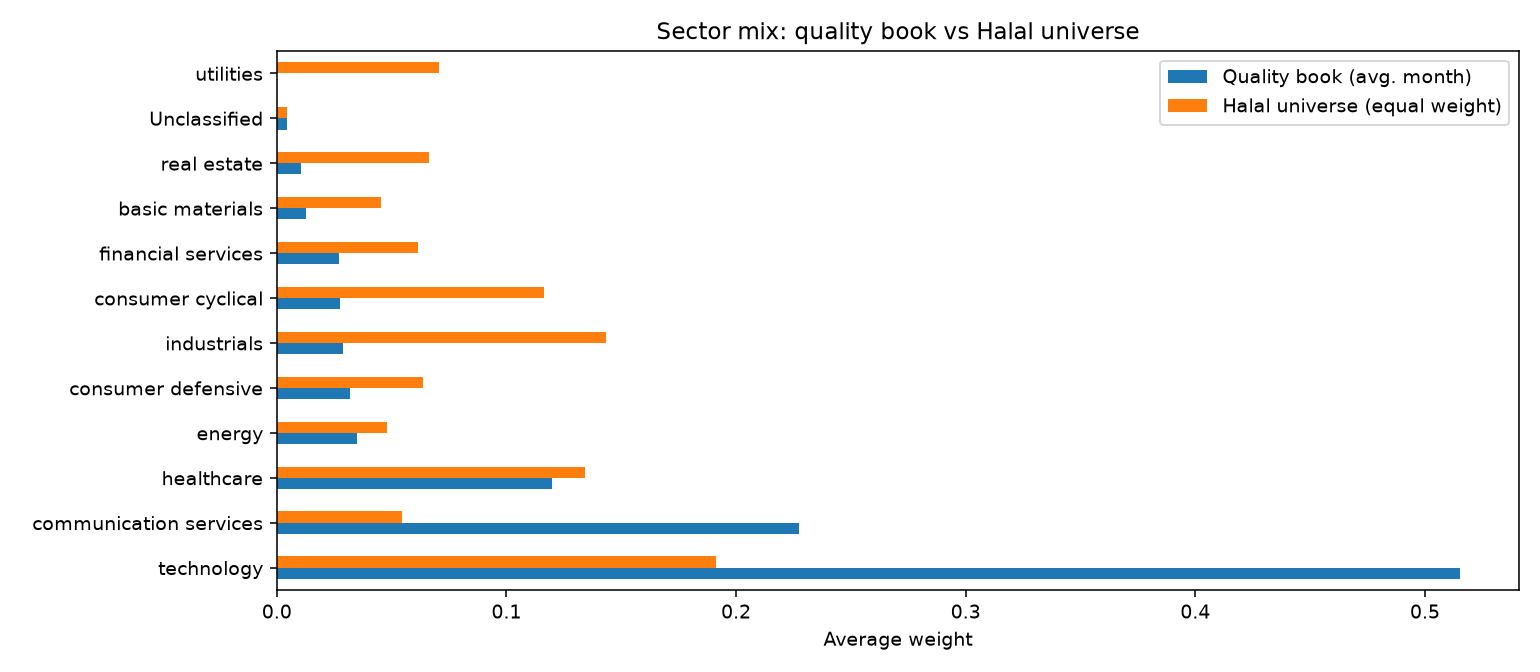
\includegraphics[width=0.92\textwidth]{figures/sector-mix.png}
\caption{Sector mix: quality book versus equal-weight Halal universe. The quality book is a tech-and-communication overweight, not a diversified Halal S\&P clone.}
\label{fig:sectors}
\end{figure}

\subsection{What we can and cannot isolate}

The leftover alpha versus SPUS is still positive after a $\beta \approx 1$ fit, so the result is not \emph{only} ``we owned SPUS.'' But SPUS itself is already Halal and tech-tilted in this window, and our book is more concentrated in the same names. Without a sector-neutral twin we cannot say how much of the 8\% SPUS alpha is FCF margin versus ``even more Apple/Nvidia/Microsoft/Alphabet/Meta than SPUS.''

The honest attribution: \textbf{stock selection inside a Halal screen produced a mega-cap quality/tech book, and that book paid in 2023--2024.}

%----------------------------------------------------------------------
\section{Limitations \& Friction}

\subsection{Turnover, slippage, and net CAGR}

Turnover is one-way: half the $\ell_1$ weight change between consecutive month-end books. Trading-cost drag assumes 10~basis points per one-way turn (a round-trip of 20~bp on the traded sleeve).

\begin{table}[htbp]
\centering
\caption{Implementation friction on the live quality book.}
\label{tab:friction}
\begin{tabular}{lr}
\toprule
Item & Value \\
\midrule
Rebalances with holdings              & 25 \\
Average names held                    & 110.9 \\
Annualized one-way turnover           & 99.9\% \\
Assumed cost per one-way trade        & 10~bp \\
Estimated annual trading-cost drag    & 0.10\% \\
CAGR gross of trading costs           & 42.43\% \\
CAGR net of trading costs             & 42.22\% \\
\bottomrule
\end{tabular}
\end{table}

Cap-weighting a broad top-half screen keeps monthly turnover low after the initial build (often a few percent a month), with a spike near March 2023 when the book expanded off the 20-name floor. Annualized one-way turnover of 99.9\% looks high because that first 100\% build and the March jump are included. Cost drag at 10~bp is only 10~bp a year---not large enough to change the headline. Real slippage on mega-caps should be tighter than 10~bp; on the smaller names in the tail it could be wider. We did not model market impact, borrow, or taxes.

\begin{figure}[htbp]
\centering
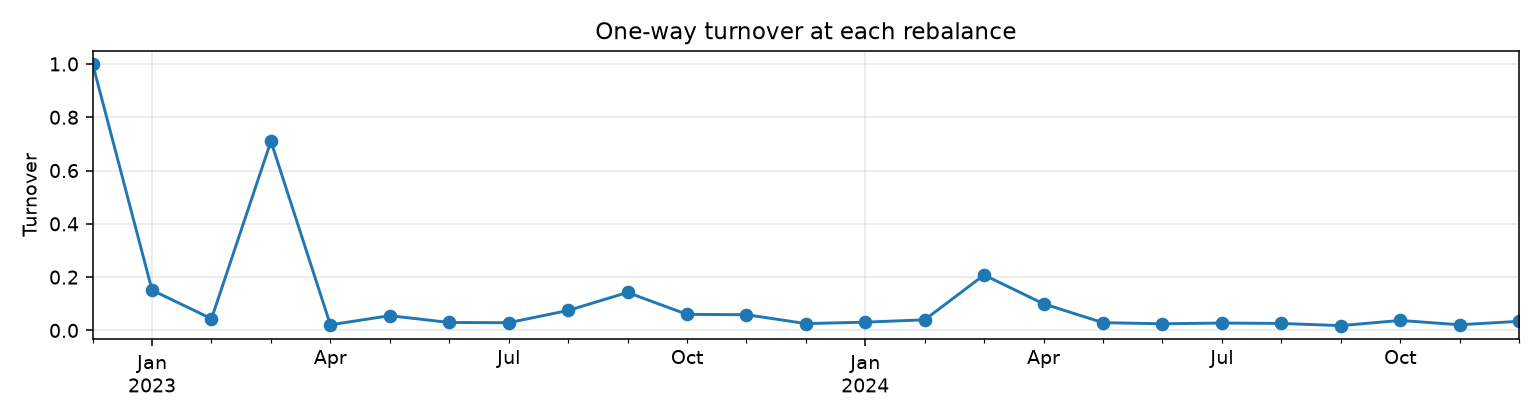
\includegraphics[width=0.92\textwidth]{figures/turnover.png}
\caption{One-way turnover at each rebalance. The first point is 100\% (book construction). After the March 2023 expansion, monthly turnover is usually well below 10\%.}
\label{fig:turnover}
\end{figure}

\subsection{Purification drag}

Impure income that may require purification is reported, not ignored. Using the library's dividend-purification helper on names that appeared in the book: \textbf{450 dividend events while held}, annualized purification drag $\approx \mathbf{0.01\%}$. That is negligible next to 42\% CAGR. Missing interest-income tags are a gap, not a 0\% drag---the 0.01\% figure is a lower bound on the names and fields we have, not a Sharia opinion that purification is optional.

\subsection{Point-in-time compliance and exits}

Screens are applied at each rebalance. Failed names are sold then. There is no intra-month compliance monitor. If a name crossed the 30\% debt line mid-month, the backtest would still hold it until month-end. That is optimistic relative to a strict daily AAOIFI process and pessimistic relative to indices that reconstitute quarterly.

Sector exclusions use the \emph{current} S\&P list and current activity labels, not the 2019 membership file. Names that were not in the S\&P in 2023 but are in it now can appear too early; names that left the index can be missing. That is survivorship and look-ahead in the universe, even though filings themselves use \texttt{filed\_date}.

\subsection{Data and construction issues}

\begin{itemize}
  \item \textbf{Short FCF history.} Yahoo annual cash-flow statements typically store a few years. First metrics date is 30~Nov~2021; first invested date is 3~Jan~2023. The 2019--2022 request is mostly unused.
  \item \textbf{FCF quality.} yfinance FCF is a pragmatic proxy until cash-flow tags live in \texttt{halalquant}. Restatements and tag mapping are not audited here.
  \item \textbf{Share-class double count.} GOOG and GOOGL are both weighted. Alphabet is overweight versus a single-listing index.
  \item \textbf{No position cap.} Three names can be a third of the book. A 5\% or 8\% cap would change both risk and 2023--2024 return.
  \item \textbf{Rule changed after seeing the data.} Cheap FCF/EV was scrapped because it lost to SPUS in this same window. 2023--2024 is partly in-sample for the live FCF-margin rule.
\end{itemize}

\subsection{What this note does not show}

There is no 2022, no 2008, no rate-hike recession, and no hold-out after the rule freeze. Quintiles are not monotonic. Sector delta explains a large part of the path. Beating SPUS in a two-year mega-cap boom is interesting; it is not evidence that AAOIFI debt caps amplify a quality premium across cycles---the original backlog question.

\subsection{Decision}

\textbf{Follow-up, do not kill, do not promote to a live book.}

Keep the idea: Halal + cash generation + cap-weight is a coherent product shape, and it was not a backtest bug. Before a second paper, freeze the rule and add (i)~SEC FCF with a longer history, (ii)~point-in-time S\&P members, (iii)~a single listing per issuer, (iv)~a sector-capped twin, and (v)~at least one down year. If the sector-capped twin still beats SPUS, the quality claim gets teeth. If it does not, this note's 42\% is mostly the 2023--2024 tech tape.

\bigskip
\noindent\textit{Reproduction.} Notebook \path{Research/papers/01-fcf-ev/code.ipynb} with \texttt{FAST\_MODE=False}, 2019-01-01 to 2024-12-31. Figures in \texttt{figures/}.

\begin{thebibliography}{9}
\bibitem{aaoifi21}
AAOIFI, ``Financial Paper (Shares and Bonds),'' Shari'ah Standard No.~21, Accounting and Auditing Organization for Islamic Financial Institutions.

\bibitem{readme}
Monterey Finance, ``Halal Quant Research Lab,'' \texttt{Research/README.md}, Phase~1 standardized white-paper structure.
\end{thebibliography}

\end{document}
